\documentclass{article}
\usepackage{graphicx} % Required for inserting images
\usepackage{amsmath}
\usepackage{pawlowski}
\usepackage{natbib}

\title{Assignment 7}
\author{Nathan Guerra}
\date{November 2024}

\begin{document}

\maketitle

\section{Summarize different techniques for taking numerical derivatives. Starting with the taylor expansion of the function f(x), derive two schemes:}
\label{intro}

Deriving our the central differencing scheme can be done by taking a taylor expansion on the function $$f(x) = \sum^{\infty}_{n=0}{\frac{f^n{(a)}}{n!}}{(x-a)^n}$$
For deriving the differencing scheme, we see what happens when x = x + h, and x = x - h. 

$$f(x+h) = f(x) + \frac{f^{1}(x)}{1!}{(x-x+h)}^{1} + \frac{f^{2}(x)}{2!}{(x-x+h)}^{2} + \frac{f^{3}(x)}{3!}{(x-x+h)}^{3}$$
This reduces down to
$$f(x+h) = f(x) + hf^{1}(x) + \frac{h^{2}}{2}f^{2}(x) + \frac{h^{3}}{6}f^{3}(x)$$
Doing the same thing for x = x - h you get.
$$f(x-h) = f(x) - hf^{1}(x) + \frac{h^{2}}{2}f^{2}(x) - \frac{h^{3}}{6}f^{3}(x)$$
Combining f(x+h) and f(x-h), such that it cancels out the second derivative for the first derivative. This can be done by subtracting f(x-h) from f(x+h).

$$f(x+h)-f(x-h)=[f(x)-f(x)]+[hf^1(x)+hf^1(x)]+[\frac{h^2}{2}{f^2(x)}-\frac{h^2}{2}{f^2(x)]+[\frac{h^3}{6}{f^3(x)}+\frac{h^3}{6}{f^3(x)}]}$$
$$f(x+h)-f(x-h)=[0]+[2hf^1(x)]+[0]+[\frac{h^3}{3}{f^3(x)}]$$ 
$$f(x+h)-f(x-h)=2hf^1(x)+\frac{h^3}{3}{f^3(x)}$$
This is what is known as the central differencing scheme. For deriving the third-order differentiation scheme,
instead of doing x = x + h, we substitute for x = x + 2h, and x = x - 2h. And repeat the same process to get. 
$$f(x+2h) = f(x) + \frac{f^{1}(x)}{1!}{(x-x+2h)}^{1} + \frac{f^{2}(x)}{2!}{(x-x+2h)}^{2} + \frac{f^{3}(x)}{3!}{(x-x+2h)}^{3}$$
Which reduces to
$$f(x+2h) = f(x) + 2hf^{1}(x) + 4h^{2}f^{2}(x) + \frac{8h^{3}}{6}f^{3}(x)$$
Substituting x = x - 2h,
$$f(x-2h) = f(x) - 2hf^{1}(x) + 4h^{2}f^{2}(x) - \frac{8h^{3}}{6}f^{3}(x)$$
Combining f(x+2h) and f(x-2h) like we did to cancel our second derivatives for the first derivatives. 
$$f(x+2h)-f(x-2h)=[f(x)-f(x)]+[2hf^1(x)+2hf^1(x)]+[2{h^2}{f^2(x)}-2{h^2}{f^2(x)]+[\frac{8h^3}{6}{f^3(x)}+\frac{8h^3}{6}{f^3(x)}]}$$
$$f(x+2h)-f(x-2h)=[0]+[4hf^1(x)]+[0]-[\frac{8h^3}{3}{f^3(x)}]$$ 
$$f(x+2h)-f(x-2h)=4hf^1(x)+\frac{8h^3}{3}{f^3(x)}$$
In order to cancel the third derivative for our third order scheme we need to multiply what we got for \\(f(x+h) - f(x-h)) by 8, and subtract it by (f(x+2h) - f(x-2h)). 
$$8(f(x+h)-f(x-h))-f(x+2h)-f(x-2h)$$
Solving for f'(x) will give you what is known as the Five-point stencil.
$$f'(x)=\frac{f(x-2h)+8f(x+h)-8f(x-h)-f(x+2h)}{12h}$$
This is a third order numerical differentiation technique.

\section{Plotting the electric potential of randomly spaced charges:}
\label{intro}
This problem wants a program that can plot a random distribution of charges using code made previously that only plotted the charges we specified instead of having the computer randomly choose for us. With this new Python program, we were given a defined function that generated the points for us, along with their randomly associated charge. These charges ranged from -1 to 1 C. The results of this code are seen below, where the heat map is of the Electric potential (\figurename~\ref{fig:contour_plot}), and the quiver plot is the directions of the Electric Field (\figurename~\ref{fig:quiver_plot}). 

\begin{figure}[h]
    \centering
    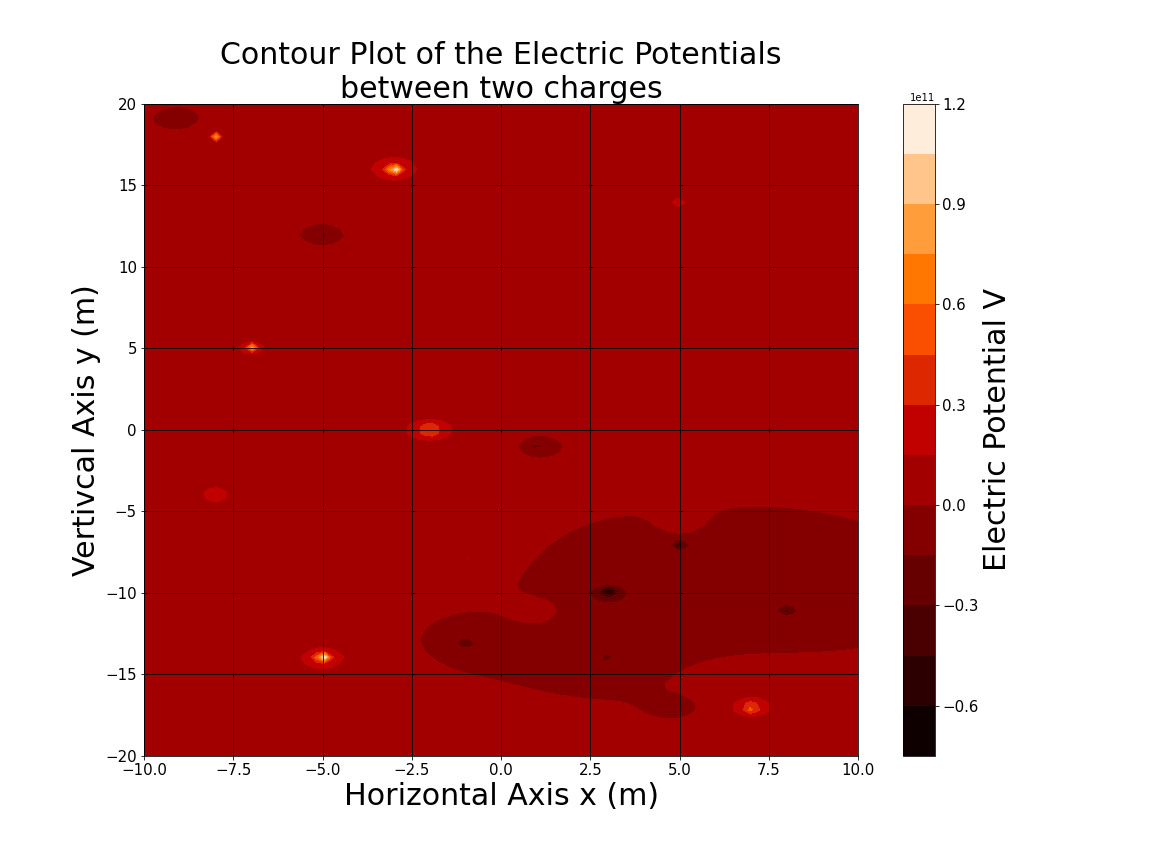
\includegraphics[width=0.8\textwidth]{potential.png}  % Specify image path and size
    \caption{Contour Plot of the Electric Potential in 2D space}
    \label{fig:contour_plot}
    \centering
    \includegraphics[width=0.8\textwidth]{efield.png}  % Specify image path and size
    \caption{Quiver Plot of the Electric Field in 2D space}
    \label{fig:quiver_plot}
\end{figure}

\section{Plotting a Harmonic Oscillator in the form of two first order differential equations:}
\label{intro}
The equations below can be associated with initial value problems. With a choice of $V_0(t)$, $y_0$, C, k and m, it is possible to solve them. Harmonic oscillators have different conditions, not damped, critically damped, overdamped, and underdamped. These 4 conditions are justified by what value of C you have. If you have a $C = 0$ (\figurename~\ref{fig:nodamp_plot}) it is not damped, if $C = \sqrt{\frac{4k}{m}}$ (\figurename~\ref{fig:crit_plot}) it is critically damped, if $C > \sqrt{\frac{4k}{m}}$ (\figurename~\ref{fig:over_plot}) it is overdamped, and if $C < \sqrt{\frac{4k}{m}}$ (\figurename~\ref{fig:under_plot}) it is underdamped.

$$\frac{dy}{dt}=V$$
$$\frac{dV}{dt}=-CV-\frac{k}{m}y$$

\section{Graphing the cyclist distance without drag:}
\label{intro}
Using the equations below with initial conditions such as $v_0=4m/s$, $P = 400W$, $m = 70kg$, and $dt = 0$ The resulting graph is place below in \figurename~\ref{fig:cycl_plot} 
$$\frac{dv}{dt}=\frac{F}{m}$$
$$\frac{dv}{dt}=\frac{P}{mv}$$


\begin{figure}[h]
    \centering
    \includegraphics[width=0.4\textwidth]{nodamping.png}  % Specify image path and size
    \caption{Harmonic Oscillator with no damping C = 0}
    \label{fig:nodamp_plot}
    \centering
    \includegraphics[width=0.4\textwidth]{criticallydamped.png}  % Specify image path and size
    \caption{Harmonic Oscillator with critically damped $C = \sqrt{\frac{4k}{m}}$ }
    \label{fig:crit_plot}
    \centering
    \includegraphics[width=0.4\textwidth]{overdamped.png}  % Specify image path and size
    \caption{Harmonic Oscillator with overdamped $C > \sqrt{\frac{4k}{m}}$}
    \label{fig:over_plot}
    \centering
    \includegraphics[width=0.4\textwidth]{underdamped.png}  % Specify image path and size
    \caption{Harmonic Oscillator with underdamped $C < \sqrt{\frac{4k}{m}}$}
    \label{fig:under_plot}
\end{figure}


\begin{figure}[h]
    \centering
    \includegraphics[width=0.4\textwidth]{cycl.png}  % Specify image path and size
    \caption{Cycling without drag figure}
    \label{fig:cycl_plot}
\end{figure}

\end{document}

